\documentclass{beamer}
\usepackage{etoolbox}\newtoggle{printable}\togglefalse{printable}
\usetheme{default}
\usecolortheme{beaver}
\usepackage{listings}
\usepackage{algpseudocode}
\graphicspath{ {./images/} }
\pdfmapfile{+sansmathaccent.map}


\title{Comp320 Research Artifact}
\author{Alastair Rayner}
\date{\today}

\begin{document}

\maketitle


\begin{frame}{Research Questions}
	\textbf{My Research questions I aim to answer}
	
	%Old
	\begin{itemize}
    		\item How does game tree search techniques compare for GVGAI? \pause
    		\item Where does each tree search technique do well in each game? \pause 
    		\item What are the strengths and weaknesses of different search techniques and how can they be improved? \pause
	\end{itemize}
	
	%New
	\begin{itemize}
		\item Can visualizing the actions an agent will take in the competition lead to  \pause
	\end{itemize}
\end{frame}






%How will this contribute to knowledge in the field
\begin{frame}{The Goal of this Research Artifact}
		\textbf{The Goal} \pause
		\begin{itemize}
			\item To create a hyper heuristic agent that has been modified from the strengths and weaknesses found in different tree search techniques. \pause
			\item The current aim is to visualize the search space of an algorithm and look for the strengths in particular games and scenarios. \pause
		\end{itemize}
\end{frame}


% What have I obtained so far
\begin{frame}{Preliminary results}
\textbf{Visualizations for the GVG-AI Competition} \pause
		\begin{itemize}
			\item One of my main focuses this far is to get visualizations rendering over the competition. \pause
			\item Being able to visualize where the agent is planning to go and finds most interesting/valuable to explore can help to creating an hyper heuristic that will search the right places(REWORD).
		\end{itemize}
\end{frame}

\begin{frame}{Demo of the GVG-AI competition and visualizations}
		\textbf{Game Example 1}
		\begin{figure}[t]
				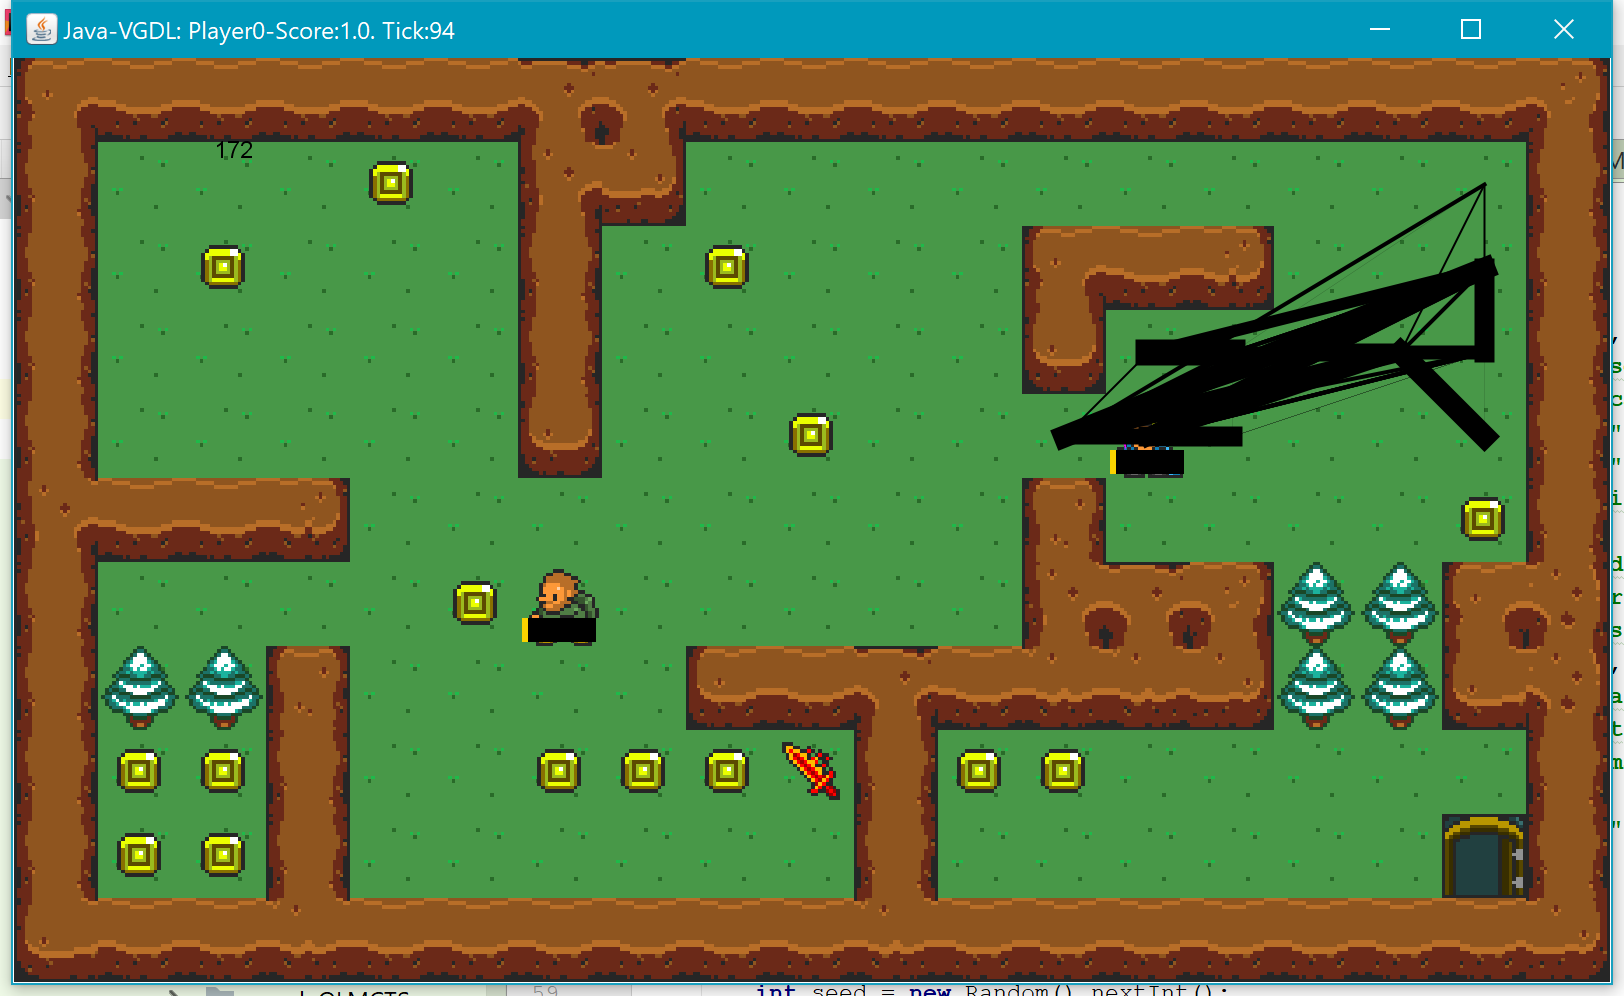
\includegraphics[width=4cm]{Game-51-1}
				
		\end{figure} 
		
		\begin{figure}[t]
				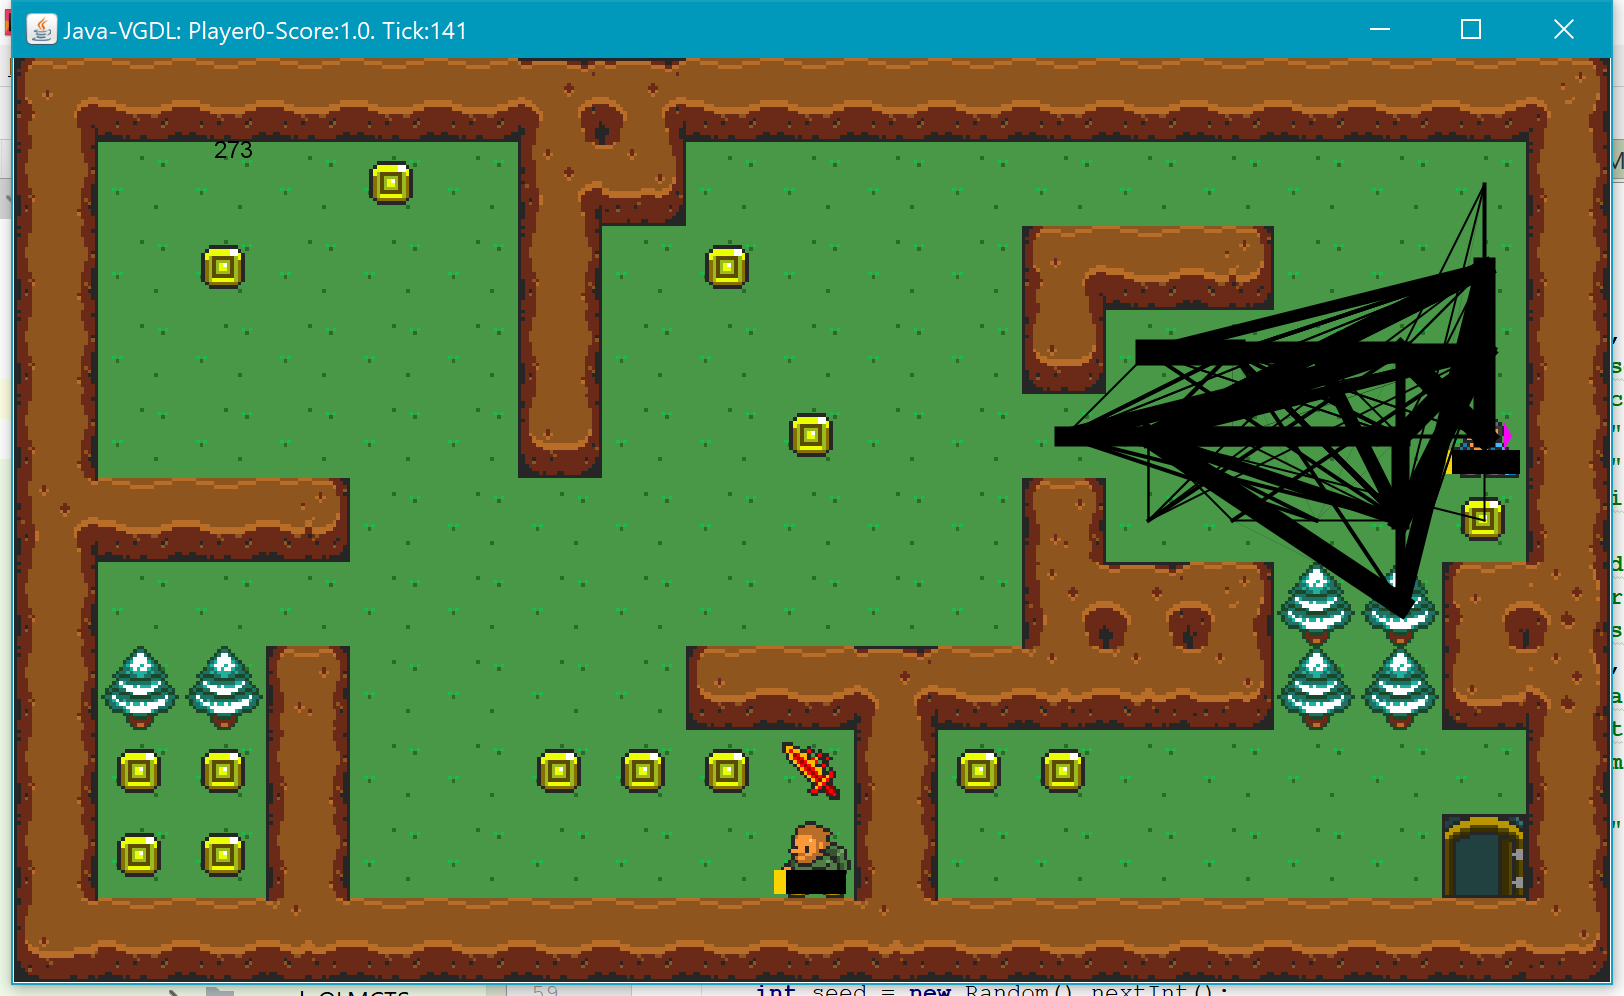
\includegraphics[width=4cm]{Game-51-2}
				
		\end{figure} \pause
		
\end{frame}

\begin{frame}{Demo of the GVG-AI competition and visualizations}
		\begin{figure}[t]
				\textbf{Live Demo}
				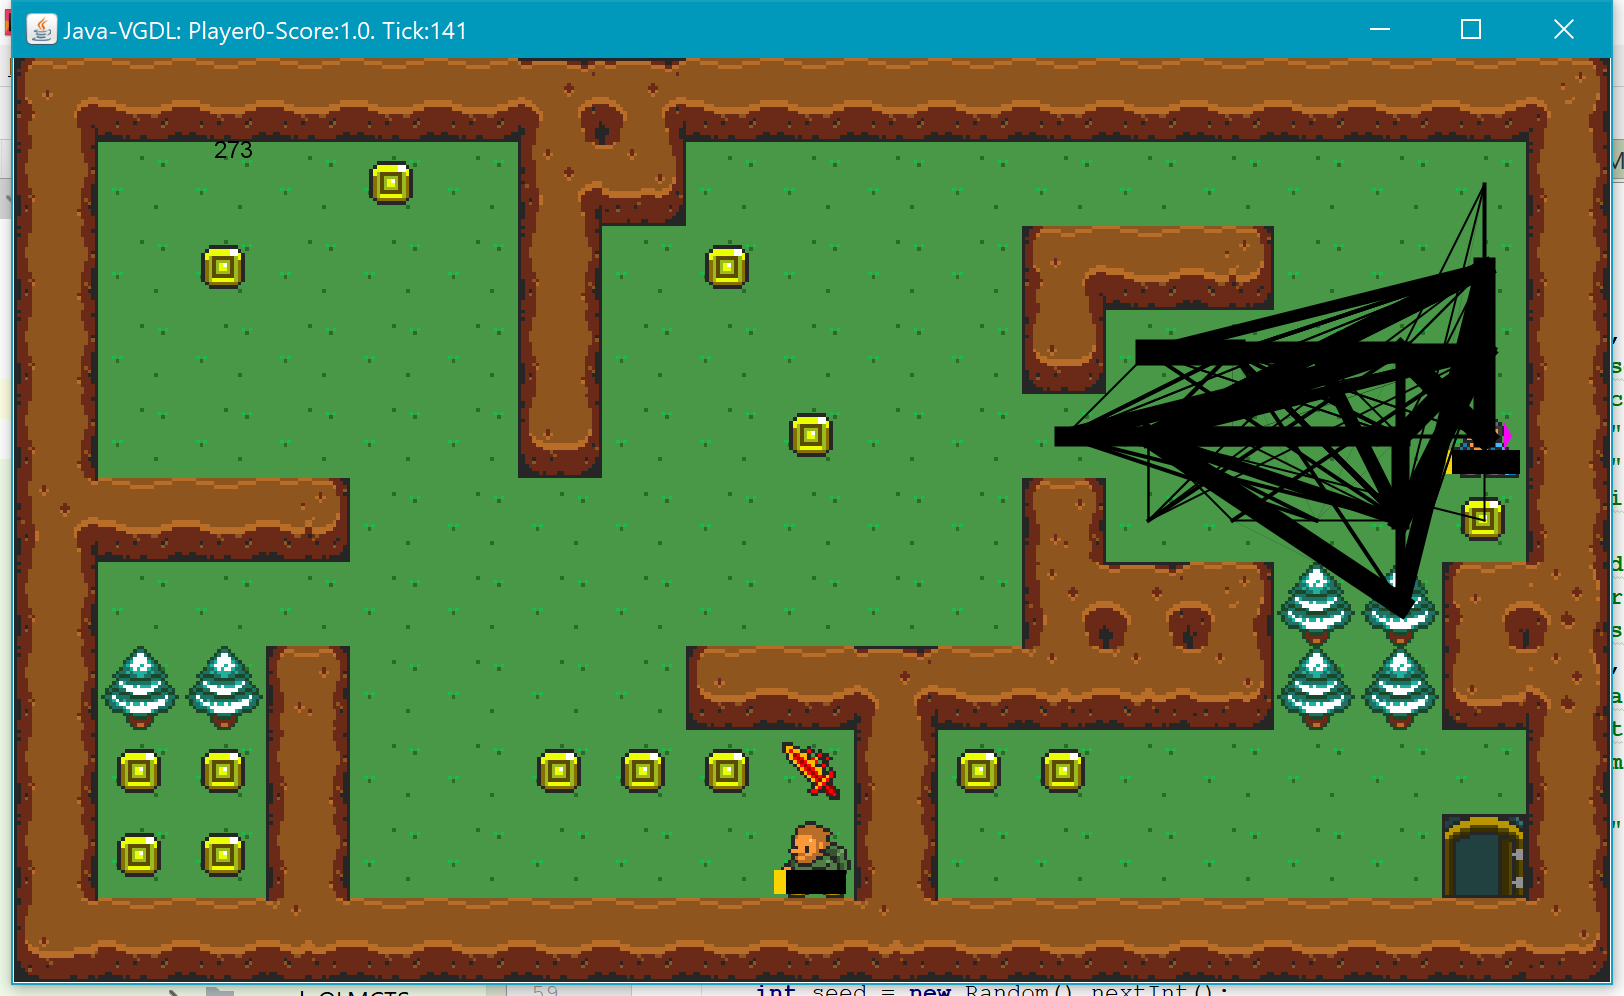
\includegraphics[width=8cm]{Game-51-2}
				\centering
		\end{figure} \pause
		
\end{frame}



\end{document}
